% Chapter: Model Architecture and Functional Decomposition
\chapter{Model Architecture and Functional Decomposition}
\label{ch:model_architecture}

\section{MTR Architectural Structure}
\label{sec:model_mtr_architecture}

The Motion Transformer (MTR) framework provides a unified approach to multimodal motion prediction, a critical task for autonomous systems. Its central principle is to model motion prediction as a joint optimization of two tasks: \textbf{global intention localization} and \textbf{local movement refinement}. In simpler terms, the model first identifies a diverse set of high-level goals or destinations for an agent and then fine-tunes the precise paths to reach those goals.

The architecture consists of two main stages:
\begin{enumerate}
    \item \textbf{Scene Context Encoding:} An encoder processes historical data from all agents and map features to build a rich understanding of the scene, including interactions between elements.
    \item \textbf{Prediction Generation:} A decoder uses a special set of "Motion Queries" to propose and refine multiple future trajectories for an agent of interest based on the encoded scene context.
\end{enumerate}

This modular, Transformer-based structure allows MTR to effectively manage the inherent uncertainty and multimodality of traffic scenarios.

\begin{figure}[htbp]
    \centering
    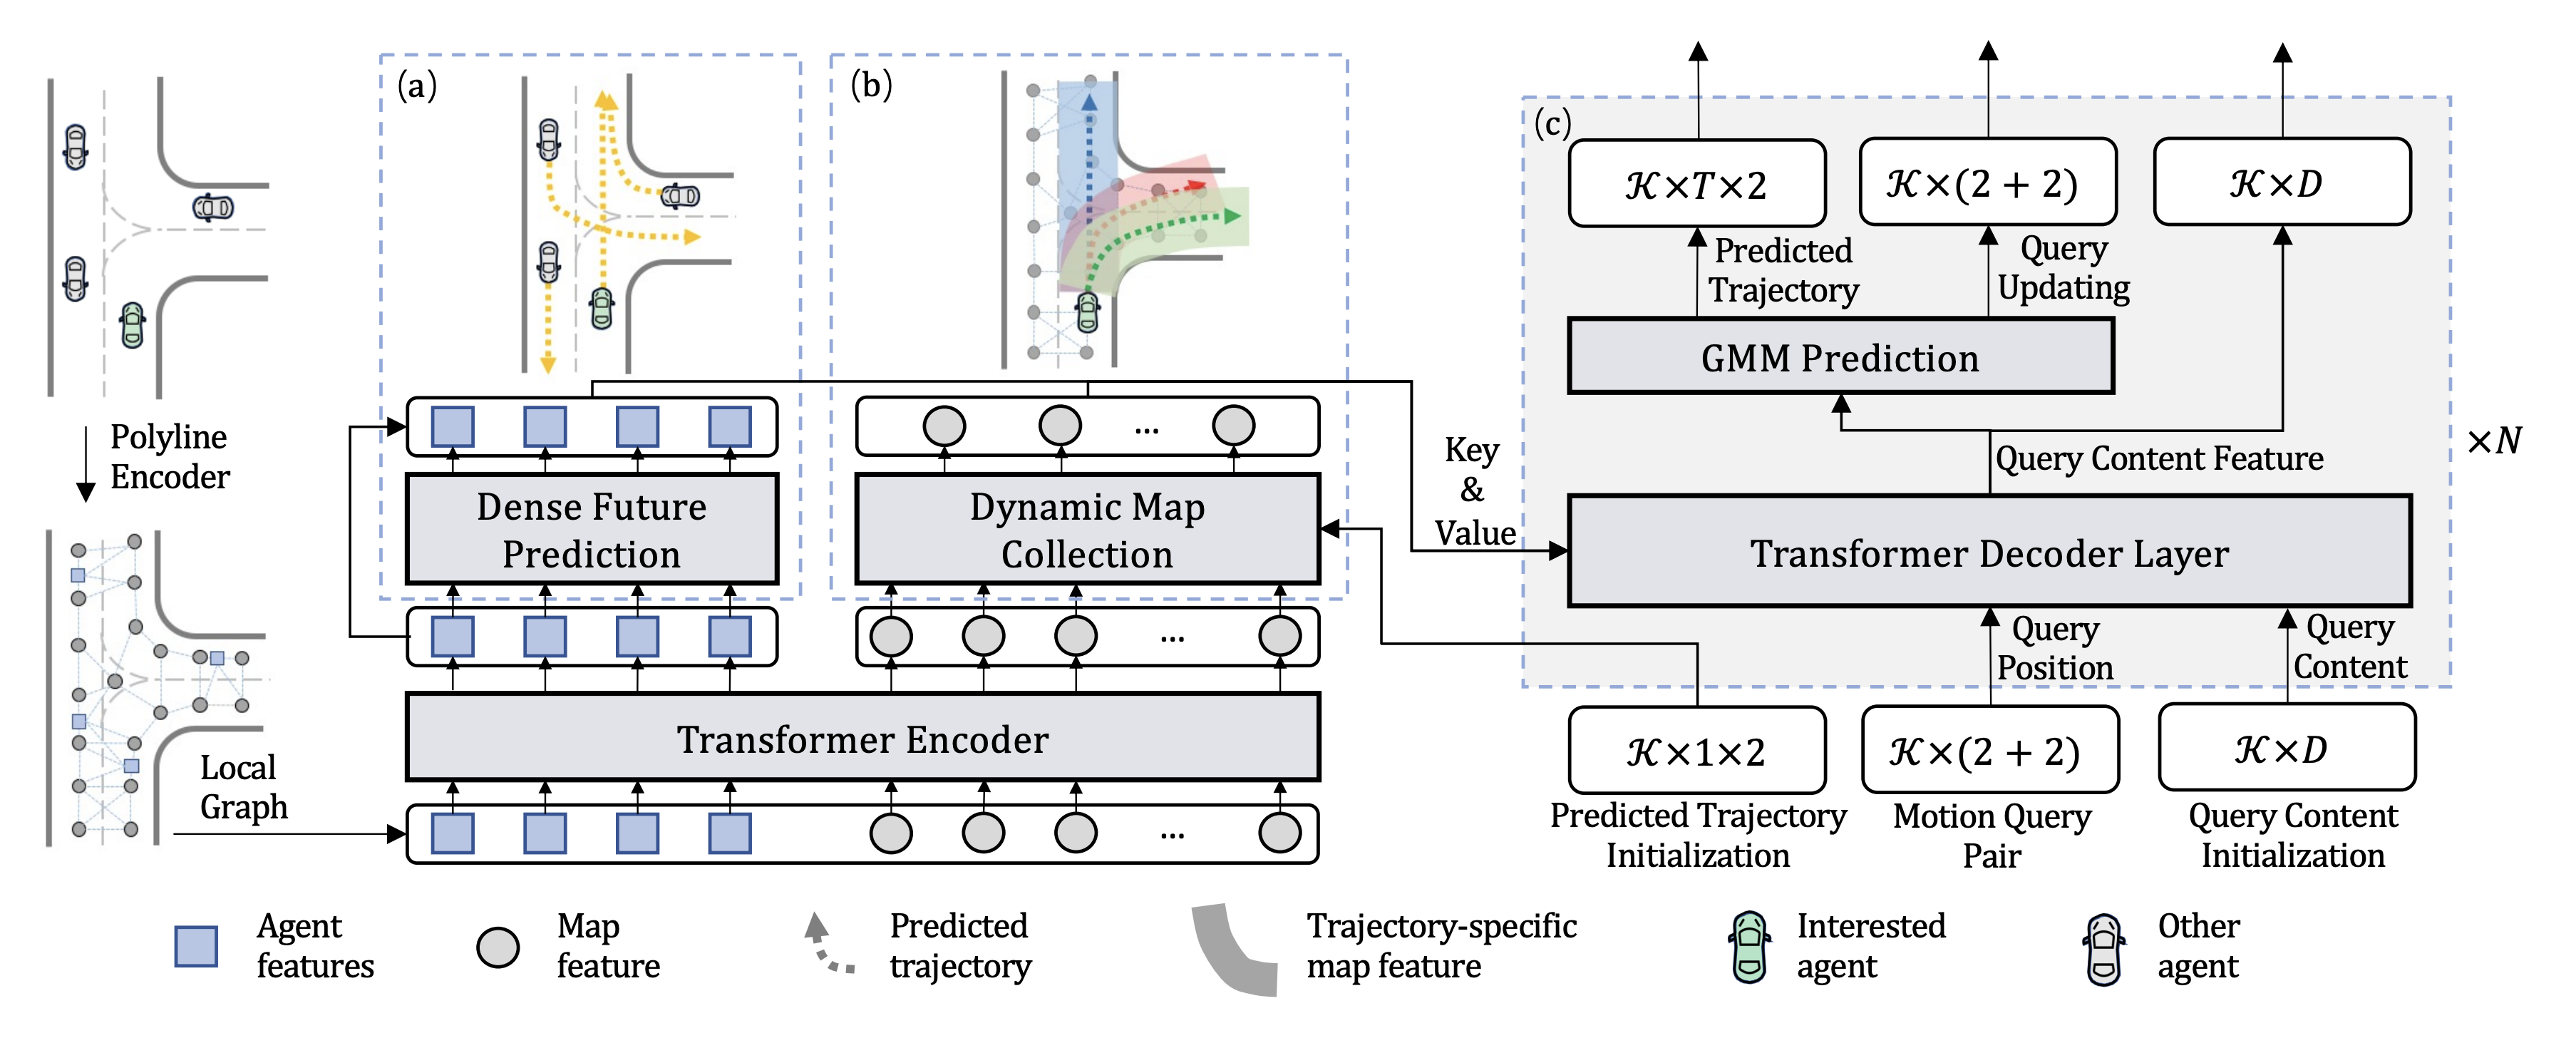
\includegraphics[width=\textwidth]{figures/mtr_overall_architecture_detail.png}
    \caption{A high-level diagram of the MTR architecture, illustrating the flow from vectorized inputs through the scene encoder and motion decoder to the final multimodal trajectory outputs. (Based on Figure 1 from \cite{Shi2022MTR}).}
    \label{fig:mtr_architecture}
\end{figure}

\section{Input Encoding}
\label{sec:model_input_encoding}
MTR represents all input data—both from agents and the map—as vectorized polylines, which are sequences of points. This method is more efficient and precise than grid-based representations like bird's-eye-view (BEV) images, as it avoids quantization errors and handles sparse map data well. PointNet-like encoders then process these polylines to generate fixed-size feature vectors for the Transformer model.

\subsection{Map Encoders}
Map features are represented as a collection of polylines, where each polyline describes a map element like a lane centerline, road boundary, or crosswalk. Each point within a polyline has attributes such as its position (x, y, z) and direction vector. A five-layer MLP processes the points of each map polyline, and a max-pooling operation aggregates this information into a single feature vector ($M_p$) for that polyline. This vector is then projected to a 256-dimensional space to match the agent feature dimensionality.

\subsection{Agent Encoders}
An agent's historical state is also treated as a polyline. The input for each agent includes its motion history (position, size, heading, velocity) over the last second. To help the model understand the data, several specific features are included:
\begin{itemize}
    \item \textbf{One-hot Category Mask:} This vector identifies the agent's type (e.g., Vehicle, Pedestrian, Cyclist). The model is designed to handle these different agent classes.
    \item \textbf{One-hot Time Embedding:} This feature explicitly encodes the timestep of each point in the history. This is crucial for the Transformer architecture, which does not otherwise have a built-in sense of sequence order.
\end{itemize}
A three-layer MLP processes these point-wise features, and max-pooling creates a 256-dimensional feature vector ($A_p$) for each agent's history.

\section{Trajectory Decoding}
\label{sec:model_decoding}
Once the inputs are encoded, the core of the MTR model performs context aggregation and generates predictions.

\subsection{Transformer Encoder Module}
The feature vectors for all agents ($A_p$) and map polylines ($M_p$) are fed into a Transformer Encoder. This module's job is to contextualize each element by modeling its interactions with its surroundings. To do this efficiently, MTR uses a \textbf{local self-attention} mechanism. Instead of having each element attend to every other element in the scene, it only attends to its $k$ nearest neighbors (e.g., $k=16$). This preserves local structure, reduces computational cost, and improves performance compared to global attention. The output of this stage is a set of context-aware feature vectors for agents ($A_{past}$) and the map ($M$).

\subsection{Dynamic Map Collection Strategy}
\label{subsec:dynamic_map_collection_strategy}
To ensure that trajectory refinement is guided by the most relevant parts of the map, MTR uses a Dynamic Map Collection strategy within its decoder. For each stage of trajectory prediction, the model identifies the $L$ map polylines (e.g., $L=128$) that are spatially closest to the current trajectory being generated. These selected map features are then used in the decoder's cross-attention mechanism, allowing the model to focus on the immediate local geometry (like lane boundaries for a lane-change maneuver) to make precise, context-aware adjustments.

\begin{figure}[htbp]
    \centering
    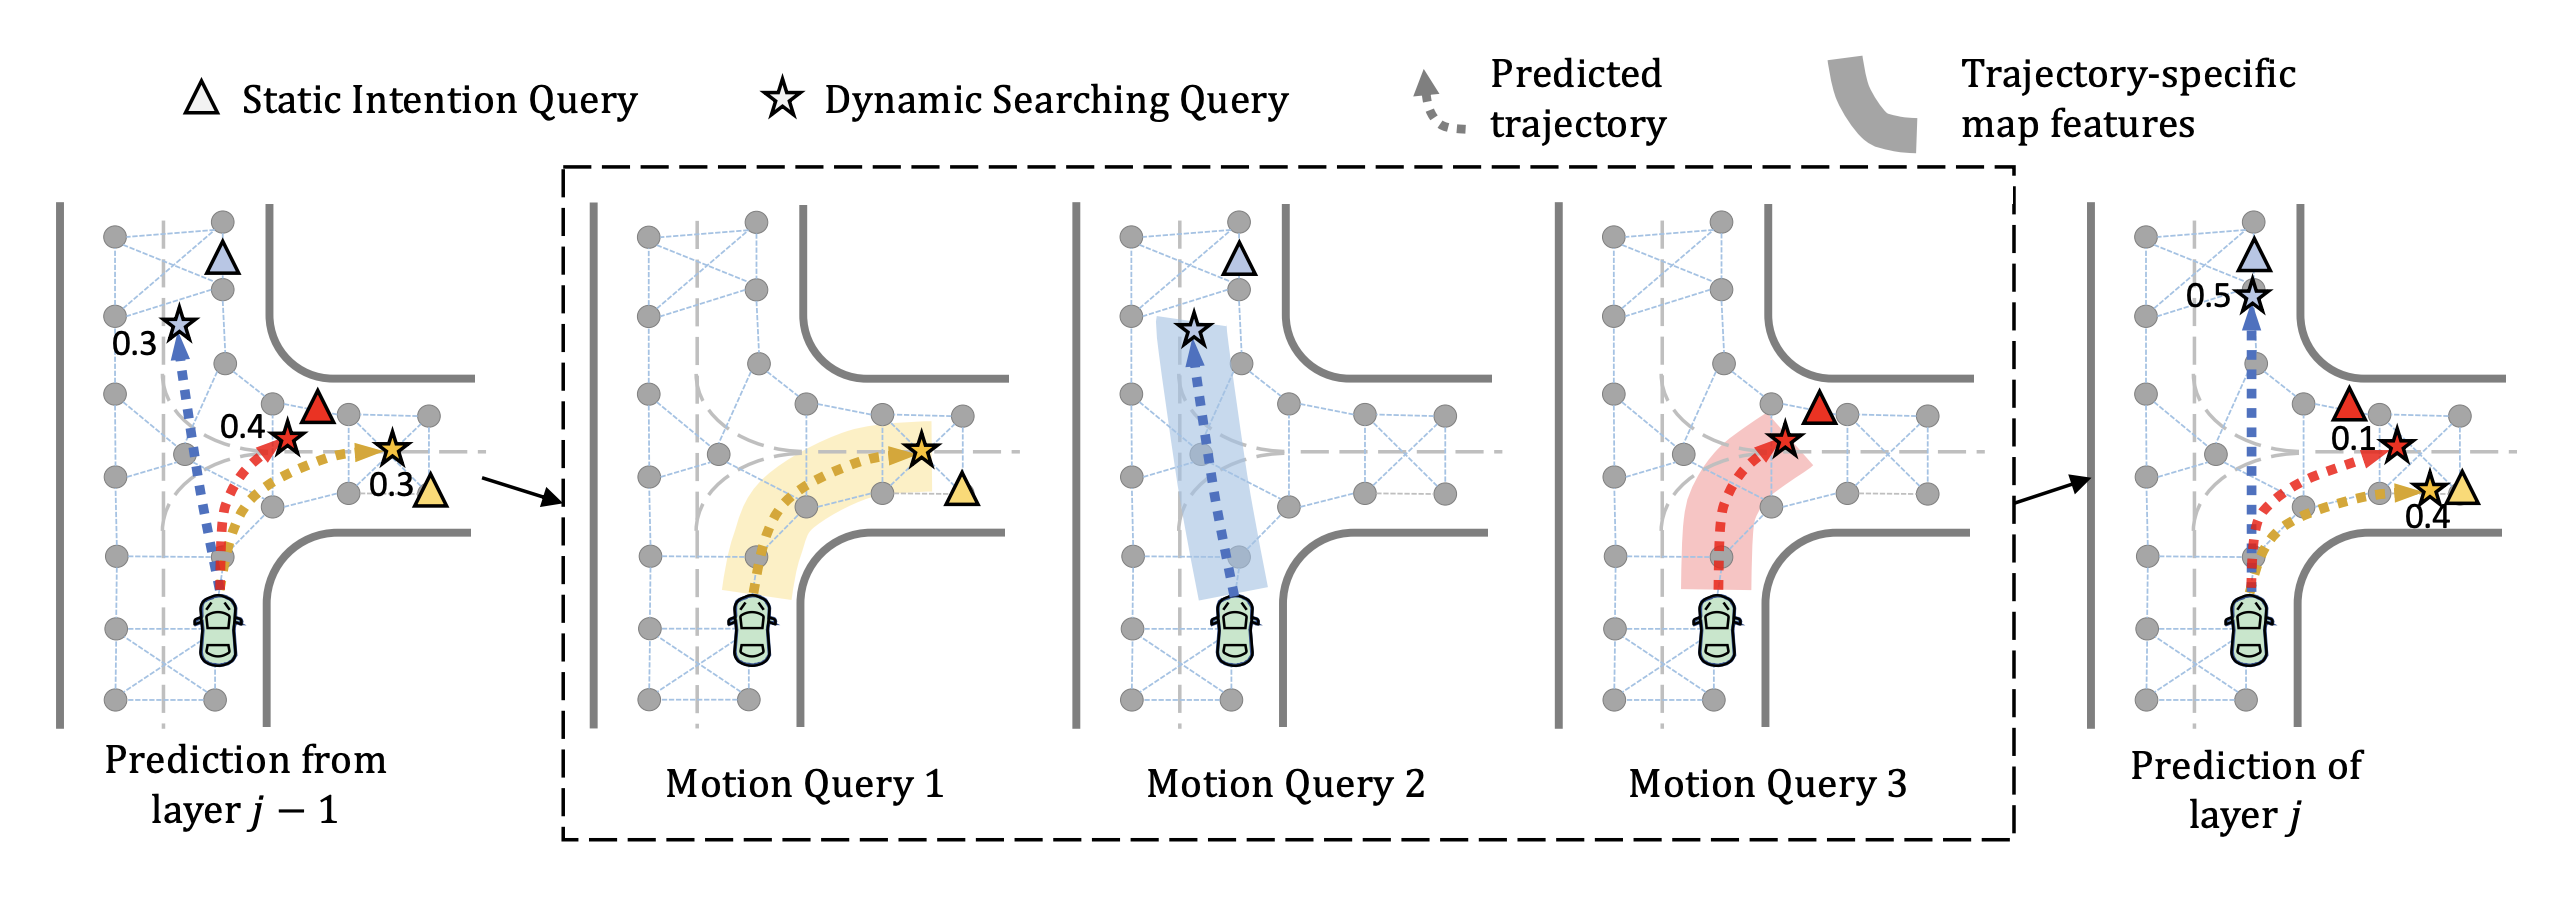
\includegraphics[width=\textwidth]{figures/dynamic_map.png}
    \caption{An illustration of the Dynamic Map Collection strategy. As a trajectory is refined (dashed line), the model selects the L closest map polylines (highlighted) to inform the next prediction step. (Based on Figure 3 from \cite{Shi2022MTR}).}
    \label{fig:dynamic_map}
\end{figure}

\subsection{Motion Decoder Module (Transformer Decoder Layer)}
The Motion Decoder generates the final trajectory predictions. Its key innovation is the use of \textbf{Motion Query Pairs} to guide this process. Each of the $K$ pairs (e.g., $K=64$) consists of a static query and a dynamic query.

\begin{itemize}
    \item \textbf{Intention-Driven Querying:} The process is driven by two types of queries:
    \begin{itemize}
        \item \textbf{Static Intention Queries ($Q_I$):} These queries act as stable anchors for different motion modes (e.g., turn left, go straight, stop). They are derived from a set of representative "intention points," which are pre-calculated by clustering the endpoints of ground-truth trajectories from the training data. Each static query specializes in a specific high-level intention, which helps disentangle the prediction of diverse behaviors and stabilizes training.
        \item \textbf{Dynamic Searching Queries ($Q_S^j$):} These queries perform the fine-grained refinement. At each decoder layer, the dynamic query is updated based on the trajectory predicted by the previous layer. It then probes the scene context (both agent and map features) to gather the specific local details needed to refine that trajectory.
    \end{itemize}
    \item \textbf{Goal-Conditioned Prediction:} The static queries ($Q_I$) enable goal-conditioned prediction. By grounding each of the $K$ prediction modes in a fixed, data-driven intention point, the model generates trajectories that are explicitly conditioned on achieving these latent goals. This synthesizes the strengths of goal-based methods (which are good at capturing multimodality) and direct-regression methods (which are good at generating refined paths).
\end{itemize}

\begin{figure}[htbp]
    \centering
    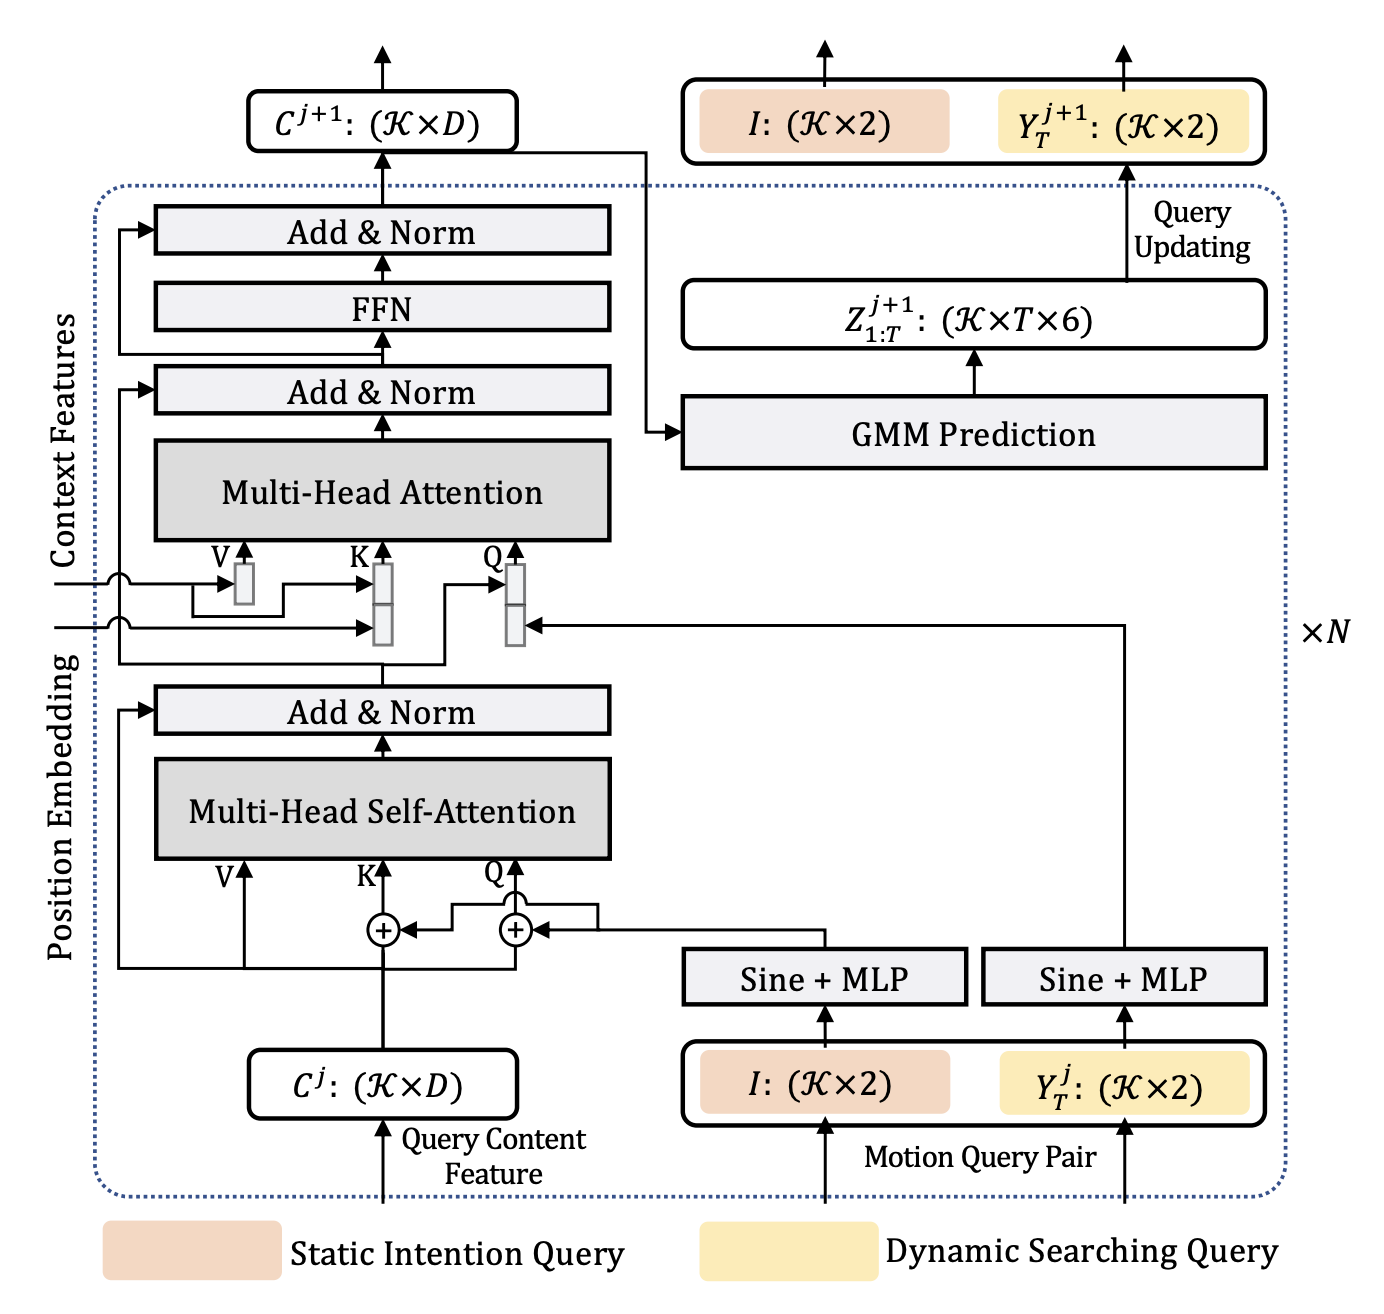
\includegraphics[width=0.6\textwidth]{figures/decoder_layer_detail.png}
    \caption{The architecture of a single Motion Decoder layer, showing how the static intention query ($Q_I$) and dynamic searching query ($Q_S^j$) interact with scene context to refine a trajectory hypothesis. (Based on Figure 2 from \cite{Shi2022MTR}).}
    \label{fig:decoder_layer}
\end{figure}

\subsection{Probabilistic Multimodal Output Generation}
To represent its multimodal predictions, MTR uses a Gaussian Mixture Model (GMM) as its final output layer. The features from the final decoder layer are passed through an MLP (prediction head) to generate the parameters for $K$ different Gaussian distributions. Each of these $K$ components represents one possible future mode and includes:
\begin{itemize}
    \item A mean trajectory (a sequence of waypoints).
    \item A probability score ($p_k$), which reflects the model's confidence in that specific mode.
\end{itemize}
This probabilistic output provides a rich distribution over plausible futures rather than a single deterministic guess.

\subsection{Iterative Query Refinement and Training}
The decoder consists of multiple stacked layers (e.g., 6 layers). This stacked structure enables an iterative refinement process. The output trajectory from layer $j-1$ is used to update the dynamic searching query ($Q_S^j$) and to guide the Dynamic Map Collection for layer $j$. Thus, an initial rough trajectory from the first layer is progressively corrected and detailed by subsequent layers, which can focus on more relevant local information.

The model is trained by comparing its $K$ predictions to the single ground-truth trajectory. A loss function guides the model to improve its predictions over time. It essentially encourages the model to assign a high probability ($p_k$) to the predicted trajectory that most closely matches the ground truth, while also moving the waypoints of that trajectory even closer to the actual path. This process can be thought of as a learned form of hypothesis testing: the queries propose $K$ hypotheses, and the training process teaches the model how to evaluate and refine them based on scene context.

\section{MTR Input-Output Formulation}
\label{sec:model_mtr_io}

At a high level, the MTR model transforms historical scene data into a set of ranked, probable future paths.

% toDO(luroess): replace figure with improved visualization of input-output visualization
\begin{figure}[htbp]
    \centering
    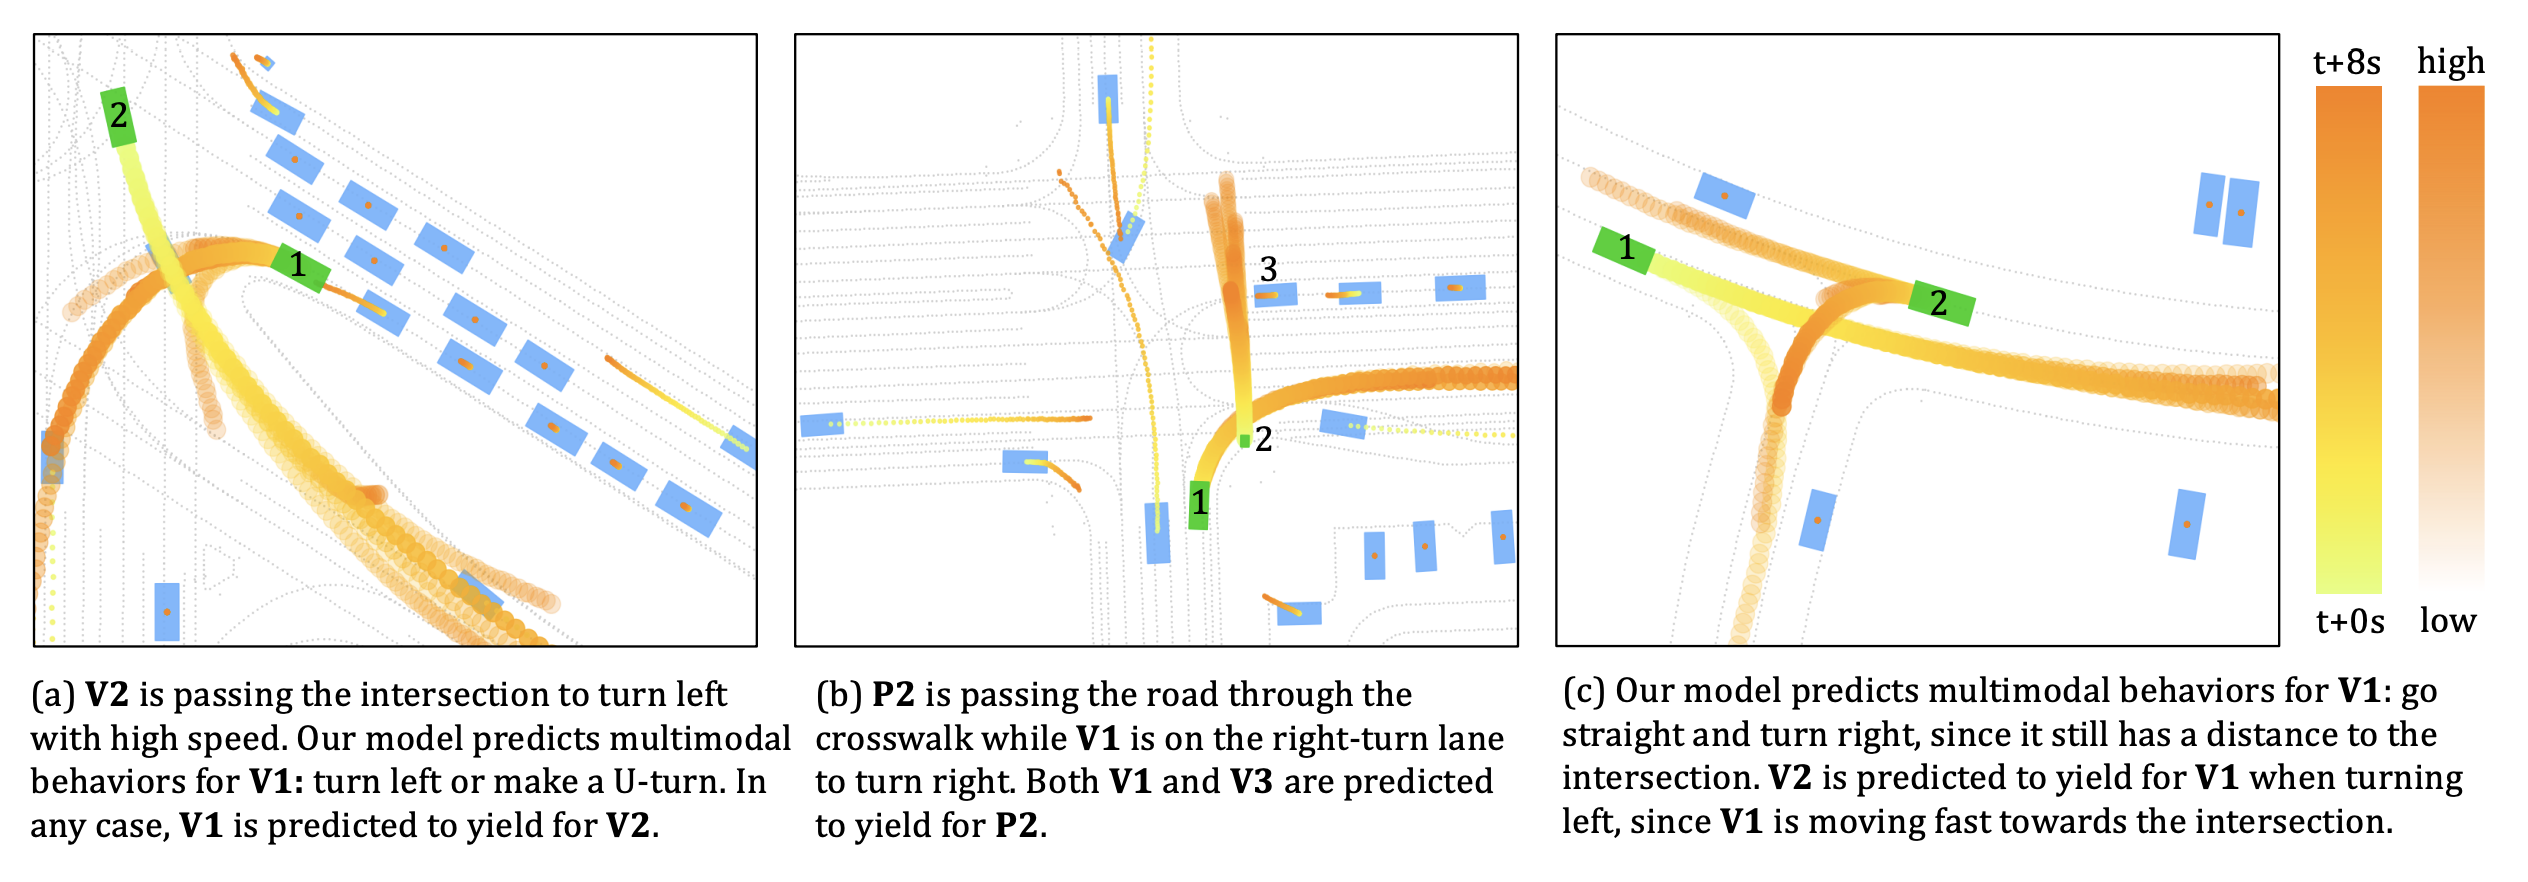
\includegraphics[width=0.9\textwidth]{figures/input_output_viz.png}
    \caption{Qualitative examples of MTR's multimodal predictions in interactive scenarios. The model generates multiple future trajectories (orange paths) for an agent of interest, with agent shwon in green. Other agents are represented by blue boxes. The examples highlight the model's ability to predict socially compliant behaviors, such as yielding to another vehicle (a), a pedestrian (b), or a fast-moving car at an intersection (c).}
    \label{fig:input_output_example}
\end{figure}

\begin{itemize}
    \item \textbf{Input Domain:} The minimum necessary input for a single agent's prediction is its historical spatiotemporal data and the features of the surrounding map environment. All input coordinates are normalized into an agent-centric frame, which makes the learning task simpler and invariant to global position and rotation. The framework is designed to process data from large-scale datasets like the Waymo Open Motion Dataset (WOMD). The model can handle various agent types, including vehicles, pedestrians, and cyclists. Within a scene, MTR processes up to 128 context agents, from which a smaller group of up to 8 "agents of interest" are designated for prediction, as specified by the WOMD benchmark. The provided documentation focuses on the MTR architecture itself and does not detail specific dataset fusion techniques (e.g., for UniTraj) or agent selection criteria (e.g., based on Kalman difficulty).

    \item \textbf{Output Domain:} The model's exact output is a set of $K$ plausible future trajectories (e.g., $K=64$) for an agent of interest over a future time horizon (e.g., 8 seconds). Each trajectory is defined by a sequence of waypoints and is associated with a probability score ($p_k$) indicating its likelihood. For evaluation against benchmarks that require a smaller number of predictions (e.g., 6), a Non-Maximum Suppression (NMS) algorithm is used to select the most likely and diverse trajectories from the initial set of $K$ proposals.
\end{itemize}

### Illustrative Scenario: Agent at a Crosswalk
To understand how the components work together, consider a vehicle approaching a crosswalk where a pedestrian is present.
\begin{enumerate}
    \item \textbf{Input and Encoding:} The model takes in the vehicle's past trajectory and the pedestrian's history, along with map polylines for the crosswalk and stop line. These are encoded into feature vectors.
    \item \textbf{Contextualization:} The Transformer Encoder's local attention mechanism allows the vehicle's feature vector to be influenced by the nearby crosswalk and pedestrian features, creating a context-aware representation. An auxiliary task predicts the likely future motion of the pedestrian, further enriching the scene context.
    \item \textbf{Decoding and Prediction:} The Motion Decoder begins its work. Static intention queries propose several plausible high-level actions, such as "yield before the crosswalk" and "proceed through".
        \begin{itemize}
            \item The "yield" hypothesis is refined. Its dynamic query focuses attention on the stop line (via Dynamic Map Collection) and the pedestrian's state.
            \item The "proceed" hypothesis is refined similarly.
        \end{itemize}
    \item \textbf{Final Output:} After iterative refinement across the decoder layers, the GMM output will reflect the context. Because the model has taken the pedestrian's presence and future path into account, the probability ($p_k$) associated with the "yield" trajectory will be high, while the "proceed" trajectory will have a low probability. This demonstrates how MTR generates contextually-aware, multimodal predictions. A visualization of this would show the vehicle's past path, the map features (lanes, crosswalk), and multiple predicted future paths, each with a different color and a displayed probability score.
\end{enumerate}

\section{Key Scientific Challenges and Model Variants}

The primary scientific challenge in motion prediction is managing the inherent uncertainty and multimodality of agent behavior in complex, interactive environments. MTR addresses this through its query-based decoder, but different versions of the model optimize for different goals.

\begin{itemize}
    \item \textbf{MTR (Standard):} The baseline model uses $K=64$ queries to generate a rich set of proposals, which are then filtered using NMS. This approach excels at capturing a wide variety of possible behaviors, leading to high performance on metrics like mean Average Precision (mAP).
    \item \textbf{MTR-e2e:} This "end-to-end" variant uses only 6 motion queries and no NMS. It is designed for scenarios where a fixed, small number of predictions is required. It uses a different training strategy better suited to the small, adaptive query set.
    \item \textbf{MTR++:} This extension tackles the more complex problem of simultaneous multi-agent prediction. It introduces a shared "Symmetric Scene Context" encoder and allows the intention queries of different agents to interact via "Mutually-Guided Intention Querying". This enables the model to produce more efficient and scene-compliant joint predictions for all agents at once.
\end{itemize}

These variants show the flexibility of the core MTR architecture in addressing the diverse challenges of motion forecasting.

\section{Conclusion}
\label{sec:conclusion}

The Motion Transformer (MTR) architecture addresses the challenge of multimodal motion prediction through its innovative design. Its core strength is the joint optimization of global intention localization and local movement refinement, which is realized through a clear encoder-decoder structure.

The architecture processes vectorized polyline inputs for agent histories and map features with PointNet-like encoders. A Transformer encoder then uses local self-attention to build a rich, contextualized scene understanding. The subsequent Motion Decoder uses its key components to generate predictions. Static intention queries ($Q_I$) provide stable, mode-specific anchors based on data-driven intention points. Dynamic searching queries ($Q_S^j$) then perform precise, context-aware refinement of these intentions. This refinement is guided by prior predictions and a dynamic map collection strategy ($\alpha(M)$). The stacked decoder layers iteratively improve the trajectories, and a final prediction head produces a probabilistic set of future paths using a Gaussian Mixture Model (GMM).

Model variants show the architecture's flexibility. MTR-e2e adapts the model for end-to-end prediction with a fixed number of outputs, while the MTR++ extension enables efficient and interactive multi-agent prediction. These architectural choices allow MTR to generate accurate, diverse, and scene-compliant trajectory forecasts. The principles of query-based prediction, iterative refinement, and adaptive context utilization are valuable paradigms for future work in autonomous navigation.